\section{Resultados}

\subsection{\label{complexidade_decod}Complexidade de decodificação BCH}

Segundo \cite{ref:algoritmo-berlekamp}, a decodificação de códigos BCH se dá em $O(n)$, $n$ sendo o tamanho de bloco empregado. Para confirmar a validade dessa afirmação, construíram-se códigos $BCH(m, 3)$, com $m \in \lbrace 4,5,...,20 \rbrace$, e mediram-se os tempos de decodificação submetendo a mesma palavra a cada um deles, com resultados ilustrados pela Figura \ref{fig:bch_decoding_is_linear}.

\begin{figure}[!hb]
	\centering
    \captionsetup{justification=centering}
	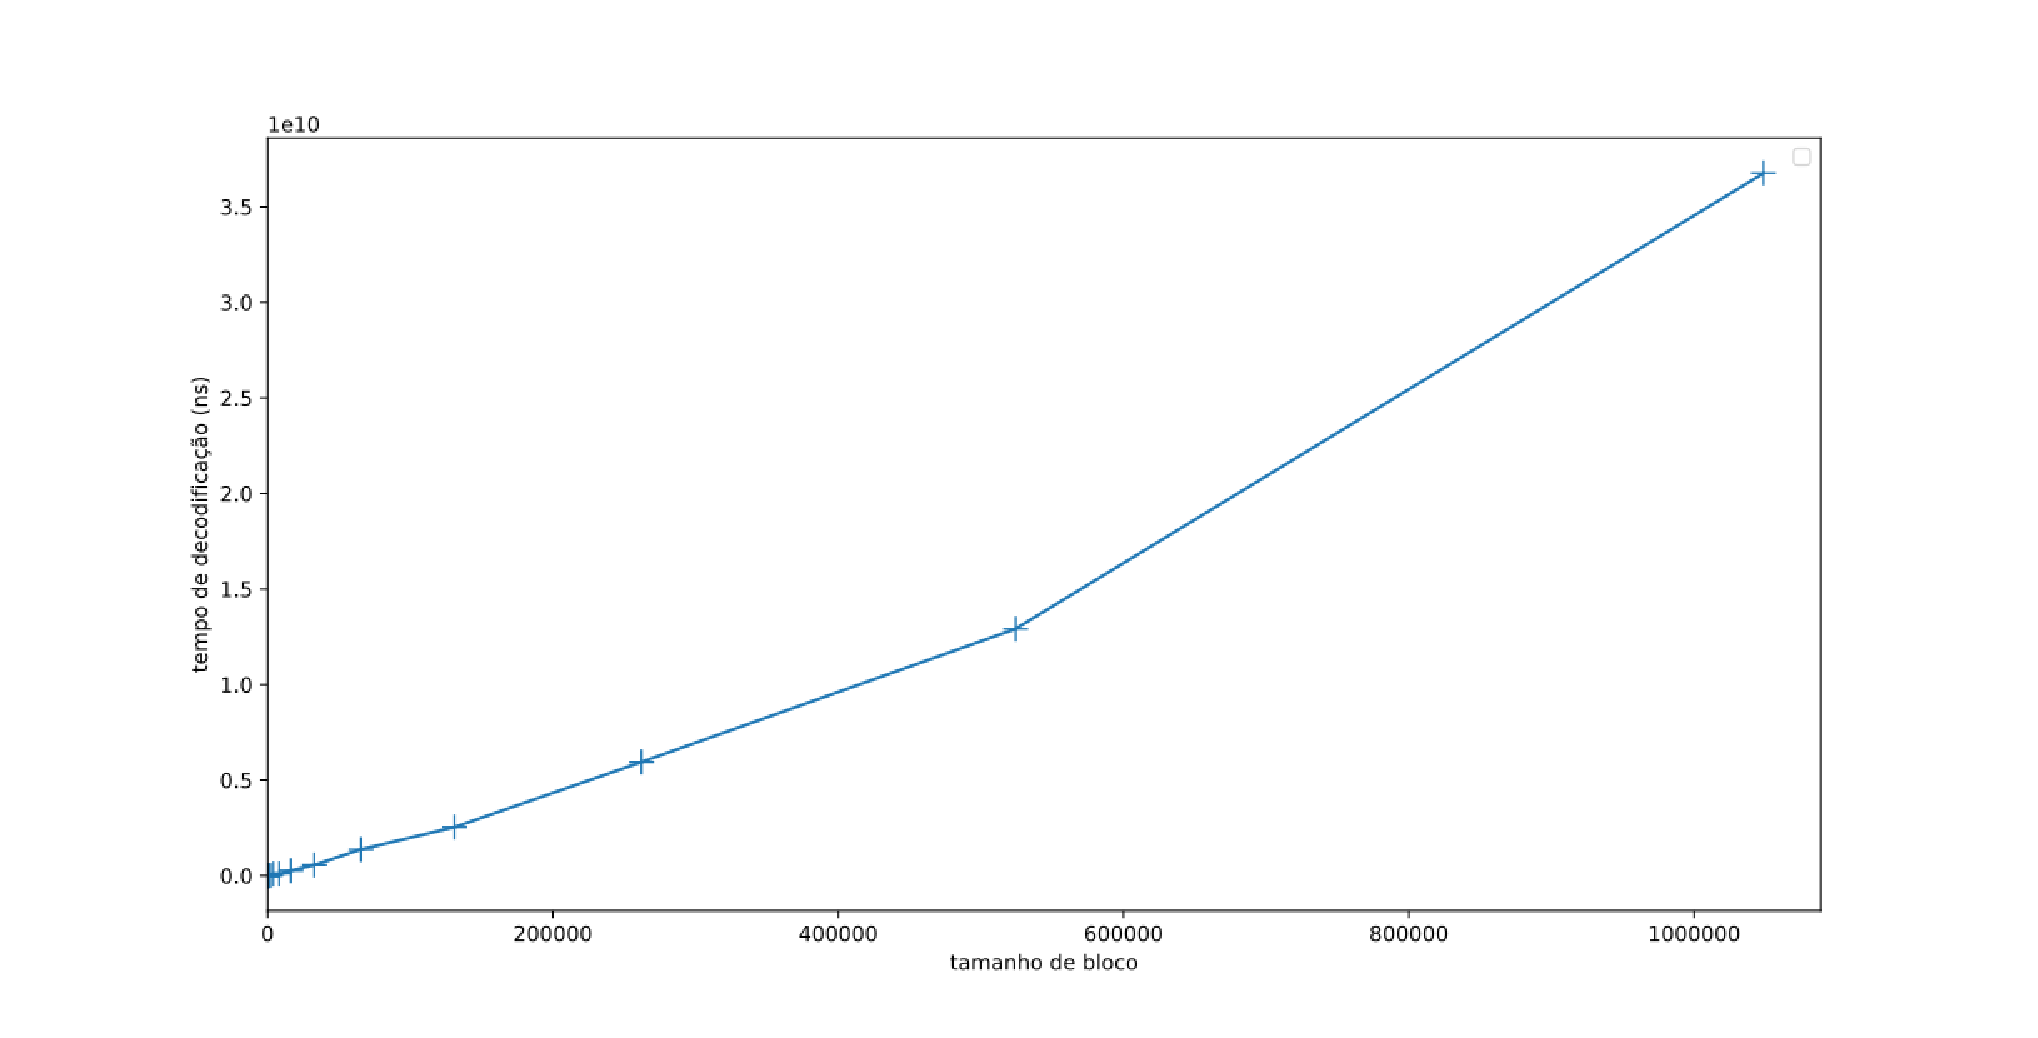
\includegraphics[scale=0.3]{floats/bch-decode-is-linear.eps}
	\caption{\label{fig:bch_decoding_is_linear}Tempo de decodificação para BCH com variados tamanhos de bloco.}
\end{figure}